\appendix
\onecolumn
\aistatstitle{Supplementary Materials}

%==============================================================================
\section{FAMILIES}
\label{app:families}

\paragraph{Poisson.}
The homogeneous Poisson process is the most fundamental SPP. It serves as a model for \emph{complete spatial
randomness} (CSR), where there is no interaction between points. It is characterized by its intensity $\lambda=\nb$:
the count $N(B)$ in any region $B$ is Poisson with mean $\lambda|B|$, counts in disjoint regions are independent.
Conditional on $N(W)=n$, points are i.i.d.\ uniform on $W$. For Poisson processes, $K(r)=\pi r^2$ and $L(r)=r$; this is why the sign of $L(r)-r$ separates clustering from regularity. Poisson is the reference against which the other families are measured.

\paragraph{Neyman--Scott.}
Let $P$ be a homogeneous Poisson \emph{parent} process with intensity $\kpar$. Each parent $p\in P$ independently
generates a Poisson($\mo$) number of \emph{offspring} points, displaced from $p$ according to a kernel $k$. Only the
offspring are observed. Conditional on $P$, the offspring form a Poisson process with intensity
\[
  \Lambda(u) = \mo \sum_{p \in P} k(u - p).
\]
We consider three Neyman--Scott processes:
\begin{enumerate}
    \item \emph{Thomas.} Displaces the offspring by an isotropic Gaussian kernel $k=\mathcal N(0,\sigma^2 I)$.
    \item \emph{Nested Thomas.} Applies the Thomas process twice: parents have Poisson($\mu_1$) children displaced with scale $\sigma_1$, and each child in turn has Poisson($\mu_2$) offspring displaced with scale $\sigma_2$.
    \item \emph{Ring.} Places the offspring uniformly on a circle of radius $\rho$ around the parent and perturbs them by $\mathcal N(0,\sigma^2 I)$, producing annular clusters.
\end{enumerate}

For all three processes, the ``visibility'' of a pattern's structure primarily depends on the \emph{overlap} of the clusters 
$\omega=\sigma\sqrt{\kpar}$ (with $\sigma = \rho$ for ring). When $\omega\ll1$ the clusters are well-separated, while $\omega\gg1$ implies overlap. The pattern approaches CSR as $\omega\to\infty$.

\paragraph{Log-Gaussian Cox.}
The log-Gaussian Cox process (LGCP) has intensity
\[
    \Lambda(u)=e^{Y(u)}
\]
for $Y$ a stationary Gaussian random field with mean $\mu_{\log}$, variance $\sigma^2$ and exponential covariance $\sigma^2 e^{-r/s}$. Points cluster where $Y$ peaks, and the pattern approaches CSR as $\sigma^2\to0$ or as $s$ shrinks relative to the spacing between points.

\paragraph{Mat\'ern hard-core.}
Let $P$ be a homogeneous Poisson \emph{proposal} process with intensity $\lambda_p$. A Mat\'ern~II process gives each point of $P$ an independent uniform mark and deletes it only if another point within the \emph{hard-core radius} $R$ has a smaller mark. This process is regular, and its patterns approach CSR as $R$ shrinks relative to the spacing between points.

\paragraph{Strauss.}
The Strauss process is a Gibbs process that penalizes, rather than forbids, close pairs. Given $N(W)=n$, its density is proportional to
\[
  (1-q)^{s_R(\pc)}, \qquad q\in[0,1),
\]
where $s_R(\pc)$ is the number of pairs closer than $R$. The \emph{inhibition strength} $q$ interpolates between the binomial process ($q\to0$, CSR given $n$) and the Gibbs hard core ($q=1$). The pattern approaches CSR as $q\to0$ or as $R$ shrinks relative to the spacing between points.

\paragraph{Cell.}
The generalized Baddeley--Silverman cell process tiles the plane with a randomly shifted, axis-aligned grid of square
cells of area $1/\nb$. Each cell independently receives $0$, $1$, or $k$ uniformly placed points, with probabilities $1/k$, $1-1/(k-1)$, and $1/(k(k-1))$, respectively. Cell counts then have mean and variance one, as for a Poisson process, so $K(r)=\pi r^2$ exactly. The cell process is therefore indistinguishable from CSR at second order despite being neither Poisson nor isotropic, which motivates the use of topological features (Section~\ref{sec:inputs}).

\paragraph{Limits between families.}
\label{app:families-limits}
Some families nearly coincide in certain regimes. As $\rho/\sigma\to0$, the ring kernel tends to the Thomas kernel, and our prior already reaches $\sigma/\rho=1$, where the annulus is largely filled; when
$\sigma_1$ is large relative to the parent spacing, the outer level is smeared out and nested Thomas resembles Thomas. Mat\'ern~II and strongly inhibited Strauss ($q\to1$) have similar pair correlations. These near equivalences account for most of the confusions between non-Poisson families (Section~\ref{sec:analysis}).

%==============================================================================
\section{SIMULATION DESIGN}
\label{app:data}

% Bank v2 (configs/v2/simulation.yaml over configs/simulation.yaml; data_v2/). Counts below are from the
% merged v2 manifests. The first bank (data/, configs/simulation.yaml) is superseded and not described here.
\paragraph{Minimal curation.}
\begin{itemize}
  \item A rule is kept only if it is a mathematical or computational limit, or excludes a degenerate setting.
        Nothing is tuned for visibility or identifiability: near-CSR patterns and patterns that two families can
        both produce are left in, because handling them is part of the problem (Section~\ref{sec:analysis}).
  \item No rule refers to departure from CSR or to any classifier; the bank is drawn on physical parameters only.
\end{itemize}

\paragraph{Sweep coordinates.}
\begin{itemize}
  \item Each $\theta$ is an i.i.d.\ draw from a constrained prior on its own seed stream, so the bank is reproducible and can be extended without moving existing draws.
  \item Every family first draws a count budget $\nb\sim\text{log-uniform}[50,950]$. The last parameter then follows from conservation of the mean count.
  \item Cluster families (Thomas, nested, ring): two independent dials, richness (points per cluster, $\ge1$) and smearing $\omega\in[0.2,8]$, the cluster scale in units of the parent spacing. Nested adds the scale ratio $\sigma_1/\sigma_2\in[1,10]$; ring adds the jitter $\sigma/\rho\in[0.05,1]$.
  \item LGCP: field variance $\sigma^2\ge0.005$ and correlation range $s\in[0.03/\sqrt{\nb},\,0.2]$. Mat\'ern~II: hard core $R\sqrt{\nb}\ge0.01$ up to the packing limit. Cell: $k\in\{2,\dots,30\}$.
  \item Strauss: simulated conditional on $n=\nb$, so the count is exact and $K$ is not needed. Inhibition strength $q=1-\gamma\sim U[0.01,1]$ ($q=1$ is the Gibbs hard core) and range $R\sqrt{n}\in[0.01,0.8]$ log-uniform, i.e.\ up to packing $0.5$, twice what Mat\'ern~II reaches.
  \item Every dial reaches down to patterns indistinguishable from CSR, so each family straddles the detection boundary.
\end{itemize}

\paragraph{Constraints.}
\begin{itemize}
  \item One degeneracy rule for every family: at least $4$ effective clusters in the window,
        $\kappa_{\rm eff}=1/(\mathrm{cv}^2-1/\nb)\ge4$, with $\mathrm{cv}=\mathrm{sd}(n)/\nb$ computed in closed form
        from $K$. For a cluster process $\mathrm{cv}^2\approx1/\nb+1/\kappa$.
        Realised cv reaches $0.46$--$0.52$ for the clustered families.
  \item Realised counts are conditioned on $n\in[20,2000]$, the range on which the null distribution of the $L$ test
        is tabulated. The condition fires for \review{$304$ of $800\,304$ simulated patterns ($0.04\%$)}, mostly
        nested at small $\nb$. Parents are simulated on a window
        buffered by 5 displacement s.d.s, to avoid edge loss.
  \item Strauss: Metropolis on the torus from a binomial start, $200$--$1000$ sweeps growing with packing;
        doubling the sweeps leaves the pair counts unchanged.
\end{itemize}

\paragraph{Data volume.}
\begin{itemize}
  \item 8 families $\times$ 50\,000 $\theta$ $\times$ 2 replicates $=$ 800\,000 patterns.
  \item Split by $\theta$ index, identical for every family: 37\,000 / 1\,000 / 12\,000 $\theta$. Both replicates of
        a $\theta$ are in the same split.
\end{itemize}


%==============================================================================
\section{MODELS AND TRAINING COST}
\label{app:models}

\begin{itemize}
  \item \new{\textbf{Persistence images} (Section~\ref{sec:model}). Following Adams et al.\ (2017), each
        (birth, death) pair becomes a Gaussian in (birth, persistence) weighted linearly by its persistence, so
        pairs on the persistence $=0$ edge are nearly weightless. A pixel holds the \emph{exact} mass of that
        surface over its box rather than a point sample, and mass outside the box is dropped rather than clamped.
        The bandwidth is one pixel ($\sigma=1$ px, so it tracks resolution) at $64\times64$. Each
        (filtration, dimension) pair gets its own box, fitted once on the training diagrams to cover $99\%$ of
        their pairs, which is why the encoders are not shared: the same pixel coordinate means something different
        in each. Coordinates enter in units of mean point spacing (pairs scaled by $\sqrt n$) and image mass is
        divided by $n$; without both, a pattern at $\nb=800$ would fill a third of the axis of one at $\nb=100$ and
        carry about seven times the mass, so resolution and dynamic range would track the regime coordinate itself.
        Images pass through $\sqrt{\cdot}$ and are then $z$-scored per channel on the training split. Alpha and Rips
        $H_0$ births are identically zero, so those are $1$-D over the persistence axis alone; DTM $H_0$ births are
        a density $2f(x)$, so DTM $H_0$ is $2$-D like every $H_1$.}
  \item \new{\textbf{Training} (Section~\ref{sec:training}). AdamW, learning rate $10^{-3}$, weight decay
        $3\times10^{-4}$, batch size $128$, at most $200$ epochs, early stopping on validation loss with patience
        $30$, and the best-validation weights restored before any prediction. One seed ($1$) per unit in the main
        results; the ablation of Section~\ref{sec:analysis} repeats every unit over seeds $\{1,2,3\}$. The
        classifier minimizes cross-entropy weighted so that each family contributes its prior's total mass, which
        under the equal prior is the inverse class count; the estimators minimize squared error on standardized
        $\log\theta$, inverted at prediction time. Early stopping is what fixes cost: ParamNet's classifier reached
        its best validation loss at epoch $17$ and stopped at $47$.}
  \item \new{\textbf{Parameter counts.} The head and encoders scale with the number of input tensors, not with the
        bank: $822\,408$ parameters for ParamNet's classifier, $526\,536$ with DTM$_{10}$ alone, $366\,600$ with
        alpha alone and $70\,728$ on the curves alone. Estimators differ only in the width of the final layer, so
        each is within $200$ parameters of its classifier.}
  \item Inputs and cost: Table~\ref{tab:cost}. \emph{Curves} is the $(4,512)$ tensor of
        $L-r,F,G,J$ (Section~\ref{sec:model}); \emph{classical} is the same curves as a feature table for the tree
        learners; \emph{ph} is the persistence summaries of one filtration's diagrams. The \new{four} network rows are the
        contrast of Section~\ref{sec:analysis}: \texttt{fusion\_curves\_alpha\_dtm10} is ParamNet,
        \texttt{nn\_curves} is the same network and trainer on the curves alone\new{, and
        \texttt{fusion\_curves\_alpha} and \texttt{fusion\_curves\_dtm10} add back one filtration each}.
  \item Hardware: the networks were trained on one GPU each, an NVIDIA A100 80GB PCIe, H100, H200 or L40S
        depending on the node the job landed on; the tree and linear models on $16$ cores of an Intel Xeon Platinum
        8268. Times are wall clock on whichever of these the unit ran on, so they compare inputs and learners only
        loosely.
\end{itemize}

\begin{table}[h]
\caption{Each model's input representation and training cost. ``Classifier'' is wall-clock seconds to train the one
$8$-way classifier until early stopping; ``Estimators'' is the same summed over the seven per-family estimators.
``Input'' names the tensors the model sees: \emph{curves} is the $(4,512)$ summary-function stack, \emph{classical}
the same curves as a feature table for the tree learners, and each filtration name a persistence summary of that
filtration's diagrams. \new{All four network rows} share one trainer and stopping rule, so their differences are the
cost of the persistence images alone. Lower is cheaper; cost is not the point of the comparison.}
\label{tab:cost}
\begin{center}
\footnotesize
% generated by paper/scripts -- do not edit; rerun python paper/scripts/make.py
\begin{tabular}{@{}lllrr@{}}
\toprule
Model & Learner & Input & Classifier (s) & Estimators (s) \\
\midrule
\texttt{fusion\_curves\_alpha\_dtm10} & nn & curves, alpha\_diameter,dtm\_k10 & 3,217 & 7,090 \\
\texttt{hgb\_classical} & hgb & classical & 414 & 132 \\
\texttt{hgb\_classical\_ph} & hgb & classical, ph\_alpha, ph\_dtm10 & 188 & 218 \\
\texttt{hgb\_ph} & hgb & ph\_alpha, ph\_dtm10 & 153 & --- \\
\texttt{linear\_classical} & linear & classical & 90 & --- \\
\texttt{nn\_curves} & nn & curves & 1,862 & 604 \\
\texttt{fusion\_curves\_alpha} & nn & curves, alpha\_diameter & 1,776 & 1,680 \\
\texttt{fusion\_curves\_dtm10} & nn & curves, dtm\_k10 & 2,081 & 1,744 \\
\bottomrule
\end{tabular}

\end{center}
\end{table}


%==============================================================================
\section{ADDITIONAL RESULTS}
\label{app:results}

The per-learner, per-family and per-filtration results behind Section~\ref{sec:analysis}.

%------------------------------------------------------------------------------
\subsection{Classification by Learner}
\label{app:classification}

Every flexible learner meets the same limit on all patterns ($0.436$--$0.452$, Table~\ref{tab:classification}), set
by the share of near-CSR patterns; the logistic regression is the floor. In the structured regime ParamNet is ahead
of the best trees, $0.754$ against $0.735$ at $\tau=0.9$, and $0.899$ against $0.862$ over the mechanisms. Adding
persistent homology helps both learners by the same amount at $\tau=0.9$: $+0.008$ [$+0.005$, $+0.010$] to the
network and $+0.009$ [$+0.007$, $+0.011$] to the trees. These intervals cover the sampling of test patterns, not of
training seeds, and each network is one seed.

\begin{table}[h]
\caption{Balanced accuracy over the eight families on the $192\,000$ test patterns. ``All'' is every pattern;
``$\tau{=}0.5$'' and ``$\tau{=}0.9$'' restrict to the structured regime at that detection power
(Section~\ref{sec:analysis}); ``Coarse'' is accuracy over the four mechanisms (CSR, clustered, regular, cell) at
$\tau{=}0.9$. Learners are named by input: ``classical'' is the summary curves, ``PH'' the persistence summaries of
the alpha and DTM$_{10}$ diagrams. Minimum contrast is penalized-contrast selection, which never selects Strauss or
cell. Intervals are within $\pm0.003$; higher is better throughout. Every learner meets the same limit on all
patterns, and ParamNet is ahead in the structured regime.}
\label{tab:classification}
\begin{center}
\footnotesize
% generated by paper/scripts -- do not edit; rerun python paper/scripts/make.py
\begin{tabular}{@{}lrrrr@{}}
\toprule
Classifier & All & $\tau{=}0.5$ & $\tau{=}0.9$ & Coarse \\
\midrule
Trees, classical + PH & 0.452 & 0.683 & 0.735 & 0.862 \\
ParamNet & 0.450 & 0.698 & 0.754 & 0.899 \\
Trees, classical & 0.447 & 0.675 & 0.726 & 0.858 \\
ParamNet, classical & 0.446 & 0.691 & 0.747 & 0.889 \\
Trees, PH & 0.436 & 0.665 & 0.719 & 0.849 \\
Logistic, classical & 0.396 & 0.583 & 0.620 & 0.783 \\
\midrule
Minimum contrast & 0.255 & 0.382 & 0.408 & 0.633 \\
\bottomrule
\end{tabular}

\end{center}
\end{table}

%------------------------------------------------------------------------------
\subsection{Per-Family Fidelity and Confusion}
\label{app:families-skill}

Table~\ref{tab:families-skill} splits the fidelity of Table~\ref{tab:main} by family. With $180$ patterns per family
at one simulation seed, per-family differences are indicative only; the pooled comparisons in the main text are the
claims. Figure~\ref{fig:confusion} is ParamNet's confusion matrix in the structured regime: $96\%$ of the confusions
between structured families stay within the same mechanism, three quarters of them among Thomas, nested and ring.

\begin{table}[h]
\caption{Skill per family, $180$ patterns each ($179$ for ring). ``$\Delta$'' is ParamNet $-$ minimum contrast on the
same patterns, given the predicted and the true family, so minimum contrast's own skill is ParamNet's minus $\Delta$.
``$^\dagger$'' marks the families with no closed-form $K$: minimum contrast never selects them, and given the true
family it falls back to the training median. Skill can exceed $1$, because on a single replicate a fit can score
better than the true model. Intervals are $95\%$ bootstrap over patterns; higher skill and positive $\Delta$ favour
ParamNet.}
\label{tab:families-skill}
\begin{center}
\footnotesize
\setlength{\tabcolsep}{3.5pt}
% generated by paper/scripts -- do not edit; rerun python paper/scripts/make.py
\begin{tabular}{@{}lrrr@{}}
\toprule
Family & ParamNet & \begin{tabular}[b]{@{}r@{}}$\Delta$\\predicted\end{tabular} & \begin{tabular}[b]{@{}r@{}}$\Delta$\\true family\end{tabular} \\
\midrule
Thomas & \begin{tabular}[t]{@{}r@{}}$1.08$\\[-2pt]{\scriptsize[$0.90$, $1.60$]}\end{tabular} & \begin{tabular}[t]{@{}r@{}}$+0.10$\\[-2pt]{\scriptsize[$+0.01$, $+0.26$]}\end{tabular} & \begin{tabular}[t]{@{}r@{}}$+0.08$\\[-2pt]{\scriptsize[$+0.00$, $+0.21$]}\end{tabular} \\
Nested & \begin{tabular}[t]{@{}r@{}}$0.87$\\[-2pt]{\scriptsize[$0.79$, $0.94$]}\end{tabular} & \begin{tabular}[t]{@{}r@{}}$-0.03$\\[-2pt]{\scriptsize[$-0.12$, $+0.06$]}\end{tabular} & \begin{tabular}[t]{@{}r@{}}$+0.08$\\[-2pt]{\scriptsize[$-0.08$, $+0.34$]}\end{tabular} \\
Ring & \begin{tabular}[t]{@{}r@{}}$0.89$\\[-2pt]{\scriptsize[$0.82$, $0.96$]}\end{tabular} & \begin{tabular}[t]{@{}r@{}}$+0.11$\\[-2pt]{\scriptsize[$-0.01$, $+0.29$]}\end{tabular} & \begin{tabular}[t]{@{}r@{}}$+0.05$\\[-2pt]{\scriptsize[$-0.05$, $+0.18$]}\end{tabular} \\
LGCP & \begin{tabular}[t]{@{}r@{}}$0.83$\\[-2pt]{\scriptsize[$0.74$, $0.92$]}\end{tabular} & \begin{tabular}[t]{@{}r@{}}$+0.18$\\[-2pt]{\scriptsize[$-0.02$, $+0.38$]}\end{tabular} & \begin{tabular}[t]{@{}r@{}}$-0.05$\\[-2pt]{\scriptsize[$-0.14$, $+0.03$]}\end{tabular} \\
Mat\'ern II & \begin{tabular}[t]{@{}r@{}}$0.99$\\[-2pt]{\scriptsize[$0.87$, $1.12$]}\end{tabular} & \begin{tabular}[t]{@{}r@{}}$-0.09$\\[-2pt]{\scriptsize[$-0.25$, $+0.04$]}\end{tabular} & \begin{tabular}[t]{@{}r@{}}$-0.12$\\[-2pt]{\scriptsize[$-0.28$, $-0.01$]}\end{tabular} \\
\midrule
Strauss$^\dagger$ & \begin{tabular}[t]{@{}r@{}}$0.94$\\[-2pt]{\scriptsize[$0.87$, $1.00$]}\end{tabular} & \begin{tabular}[t]{@{}r@{}}$+0.55$\\[-2pt]{\scriptsize[$+0.40$, $+0.70$]}\end{tabular} & \begin{tabular}[t]{@{}r@{}}$+0.86$\\[-2pt]{\scriptsize[$+0.75$, $+0.97$]}\end{tabular} \\
Cell$^\dagger$ & \begin{tabular}[t]{@{}r@{}}$0.91$\\[-2pt]{\scriptsize[$0.50$, $1.34$]}\end{tabular} & \begin{tabular}[t]{@{}r@{}}$+2.81$\\[-2pt]{\scriptsize[$+1.13$, $+6.20$]}\end{tabular} & \begin{tabular}[t]{@{}r@{}}$+1.22$\\[-2pt]{\scriptsize[$+0.78$, $+2.14$]}\end{tabular} \\
\bottomrule
\end{tabular}

\end{center}
\end{table}

\begin{figure}[h]
\centering
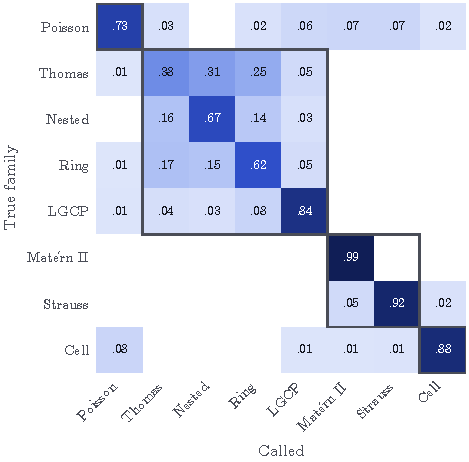
\includegraphics{figs/v2/f3_confusion}
\caption{Confusion matrix of ParamNet in the structured regime ($\tau=0.9$), rows normalized: the share of each true
family assigned to each family; blank cells are below $0.005$. Boxes: the mechanisms (CSR, clustered, regular, cell).
Confusions stay within the mechanism, mostly among Thomas, nested and ring, which produce the same patterns over part
of their parameter spaces.}
\label{fig:confusion}
\end{figure}

%------------------------------------------------------------------------------
\subsection{Per-Family Estimation Error}
\label{app:estimation}

\new{Every estimator of every family, given the true family, by
$\mathrm{RMSE}(\log\theta)/\mathrm{s.d.}$ averaged over the family's targets. Minimum contrast is fitted to the same
family's closed-form $K$, so the comparison isolates the estimate and not the selection; it has no regime columns
because it is reported on all patterns only.}

\begin{table}[h]
\caption{\new{Estimation error per family and estimator, given the true family. Cells are
$\mathrm{RMSE}(\log\theta)/\mathrm{s.d.}$ averaged over the family's targets, where $1$ is the error of predicting
the training mean. ``Val'' is the validation split; ``All'' is every test pattern; ``$\tau{=}0.5$'' and
``$\tau{=}0.9$'' restrict to the structured regime at that detection power. ``$\star$'' marks the lowest validation
error, the estimator a per-family selection rule would pick. Intervals are $95\%$ over test $\theta$; lower is
better. Every learner beats minimum contrast on every family.}}
\label{tab:estimation}
\begin{center}
\scriptsize
% generated by paper/scripts -- do not edit; rerun python paper/scripts/make.py
\begin{tabular}{@{}llrrrr@{}}
\toprule
Family & Estimator ($\star$ = best on val) & Val & All & $\tau{=}0.5$ & $\tau{=}0.9$ \\
\midrule
Thomas & \texttt{fusion\_curves\_alpha\_dtm10} $\star$ & 0.742 & 0.739 {\scriptsize [0.733, 0.746]} & 0.548 {\scriptsize [0.538, 0.558]} & 0.407 {\scriptsize [0.397, 0.417]} \\
Thomas & \texttt{fusion\_curves\_dtm10} & 0.743 & 0.741 {\scriptsize [0.734, 0.748]} & 0.559 {\scriptsize [0.549, 0.569]} & 0.426 {\scriptsize [0.416, 0.437]} \\
Thomas & \texttt{fusion\_curves\_alpha} & 0.745 & 0.741 {\scriptsize [0.735, 0.748]} & 0.556 {\scriptsize [0.546, 0.566]} & 0.427 {\scriptsize [0.416, 0.438]} \\
Thomas & \texttt{nn\_curves} & 0.746 & 0.741 {\scriptsize [0.735, 0.748]} & 0.553 {\scriptsize [0.543, 0.563]} & 0.415 {\scriptsize [0.404, 0.426]} \\
Thomas & \texttt{hgb\_classical\_ph} & 0.750 & 0.744 {\scriptsize [0.738, 0.750]} & 0.553 {\scriptsize [0.542, 0.563]} & 0.421 {\scriptsize [0.409, 0.430]} \\
Thomas & \texttt{hgb\_classical} & 0.752 & 0.745 {\scriptsize [0.739, 0.751]} & 0.555 {\scriptsize [0.545, 0.565]} & 0.425 {\scriptsize [0.414, 0.435]} \\
Thomas & min.\ contrast (tuned) & --- & 1.762 & --- & --- \\
Nested & \texttt{fusion\_curves\_alpha} & 0.729 & 0.717 {\scriptsize [0.711, 0.724]} & 0.638 {\scriptsize [0.631, 0.646]} & 0.570 {\scriptsize [0.564, 0.577]} \\
Nested & \texttt{fusion\_curves\_dtm10} $\star$ & 0.728 & 0.717 {\scriptsize [0.712, 0.725]} & 0.636 {\scriptsize [0.629, 0.644]} & 0.571 {\scriptsize [0.563, 0.578]} \\
Nested & \texttt{fusion\_curves\_alpha\_dtm10} & 0.729 & 0.719 {\scriptsize [0.714, 0.726]} & 0.639 {\scriptsize [0.631, 0.647]} & 0.571 {\scriptsize [0.564, 0.578]} \\
Nested & \texttt{nn\_curves} & 0.731 & 0.719 {\scriptsize [0.714, 0.726]} & 0.642 {\scriptsize [0.635, 0.649]} & 0.576 {\scriptsize [0.569, 0.583]} \\
Nested & \texttt{hgb\_classical\_ph} & 0.735 & 0.724 {\scriptsize [0.719, 0.731]} & 0.641 {\scriptsize [0.634, 0.649]} & 0.573 {\scriptsize [0.565, 0.580]} \\
Nested & \texttt{hgb\_classical} & 0.740 & 0.726 {\scriptsize [0.721, 0.733]} & 0.647 {\scriptsize [0.641, 0.655]} & 0.580 {\scriptsize [0.572, 0.587]} \\
Nested & min.\ contrast (tuned) & --- & 2.250 & --- & --- \\
LGCP & \texttt{hgb\_classical} & 0.542 & 0.541 {\scriptsize [0.536, 0.545]} & 0.356 {\scriptsize [0.348, 0.365]} & 0.279 {\scriptsize [0.269, 0.289]} \\
LGCP & \texttt{fusion\_curves\_alpha\_dtm10} $\star$ & 0.540 & 0.541 {\scriptsize [0.536, 0.546]} & 0.364 {\scriptsize [0.355, 0.372]} & 0.289 {\scriptsize [0.280, 0.299]} \\
LGCP & \texttt{nn\_curves} & 0.542 & 0.541 {\scriptsize [0.536, 0.546]} & 0.366 {\scriptsize [0.357, 0.374]} & 0.301 {\scriptsize [0.290, 0.311]} \\
LGCP & \texttt{hgb\_classical\_ph} & 0.543 & 0.541 {\scriptsize [0.537, 0.546]} & 0.359 {\scriptsize [0.350, 0.367]} & 0.283 {\scriptsize [0.273, 0.293]} \\
LGCP & \texttt{fusion\_curves\_alpha} & 0.541 & 0.541 {\scriptsize [0.537, 0.546]} & 0.365 {\scriptsize [0.356, 0.373]} & 0.293 {\scriptsize [0.283, 0.303]} \\
LGCP & \texttt{fusion\_curves\_dtm10} & 0.544 & 0.542 {\scriptsize [0.537, 0.547]} & 0.363 {\scriptsize [0.354, 0.371]} & 0.295 {\scriptsize [0.284, 0.306]} \\
LGCP & min.\ contrast (tuned) & --- & 0.873 & --- & --- \\
Mat\'ern II & \texttt{fusion\_curves\_alpha} & 0.238 & 0.233 {\scriptsize [0.230, 0.236]} & 0.114 {\scriptsize [0.111, 0.117]} & 0.089 {\scriptsize [0.087, 0.092]} \\
Mat\'ern II & \texttt{nn\_curves} & 0.240 & 0.233 {\scriptsize [0.230, 0.236]} & 0.103 {\scriptsize [0.101, 0.105]} & 0.084 {\scriptsize [0.082, 0.086]} \\
Mat\'ern II & \texttt{hgb\_classical\_ph} $\star$ & 0.238 & 0.234 {\scriptsize [0.231, 0.237]} & 0.109 {\scriptsize [0.106, 0.112]} & 0.088 {\scriptsize [0.086, 0.090]} \\
Mat\'ern II & \texttt{hgb\_classical} & 0.240 & 0.235 {\scriptsize [0.232, 0.238]} & 0.110 {\scriptsize [0.108, 0.113]} & 0.089 {\scriptsize [0.086, 0.092]} \\
Mat\'ern II & \texttt{fusion\_curves\_alpha\_dtm10} & 0.241 & 0.236 {\scriptsize [0.233, 0.239]} & 0.116 {\scriptsize [0.113, 0.119]} & 0.090 {\scriptsize [0.088, 0.093]} \\
Mat\'ern II & \texttt{fusion\_curves\_dtm10} & 0.245 & 0.243 {\scriptsize [0.240, 0.246]} & 0.137 {\scriptsize [0.134, 0.140]} & 0.118 {\scriptsize [0.116, 0.121]} \\
Mat\'ern II & min.\ contrast (tuned) & --- & 0.315 & --- & --- \\
Ring & \texttt{fusion\_curves\_dtm10} & 0.706 & 0.709 {\scriptsize [0.702, 0.716]} & 0.601 {\scriptsize [0.591, 0.611]} & 0.457 {\scriptsize [0.448, 0.466]} \\
Ring & \texttt{fusion\_curves\_alpha} $\star$ & 0.703 & 0.709 {\scriptsize [0.702, 0.716]} & 0.599 {\scriptsize [0.590, 0.607]} & 0.449 {\scriptsize [0.439, 0.459]} \\
Ring & \texttt{fusion\_curves\_alpha\_dtm10} & 0.705 & 0.710 {\scriptsize [0.703, 0.717]} & 0.599 {\scriptsize [0.590, 0.608]} & 0.461 {\scriptsize [0.451, 0.470]} \\
Ring & \texttt{hgb\_classical\_ph} & 0.705 & 0.710 {\scriptsize [0.703, 0.717]} & 0.590 {\scriptsize [0.581, 0.600]} & 0.436 {\scriptsize [0.428, 0.445]} \\
Ring & \texttt{nn\_curves} & 0.707 & 0.711 {\scriptsize [0.704, 0.718]} & 0.605 {\scriptsize [0.596, 0.614]} & 0.457 {\scriptsize [0.449, 0.466]} \\
Ring & \texttt{hgb\_classical} & 0.715 & 0.715 {\scriptsize [0.708, 0.722]} & 0.604 {\scriptsize [0.595, 0.613]} & 0.462 {\scriptsize [0.453, 0.471]} \\
Ring & min.\ contrast (tuned) & --- & 1.475 & --- & --- \\
Cell & \texttt{hgb\_classical\_ph} $\star$ & 0.132 & 0.137 {\scriptsize [0.135, 0.140]} & 0.137 {\scriptsize [0.135, 0.140]} & 0.137 {\scriptsize [0.135, 0.140]} \\
Cell & \texttt{fusion\_curves\_dtm10} & 0.137 & 0.141 {\scriptsize [0.139, 0.143]} & 0.141 {\scriptsize [0.139, 0.143]} & 0.141 {\scriptsize [0.139, 0.143]} \\
Cell & \texttt{fusion\_curves\_alpha\_dtm10} & 0.138 & 0.143 {\scriptsize [0.140, 0.145]} & 0.143 {\scriptsize [0.140, 0.145]} & 0.143 {\scriptsize [0.140, 0.145]} \\
Cell & \texttt{fusion\_curves\_alpha} & 0.148 & 0.153 {\scriptsize [0.151, 0.156]} & 0.153 {\scriptsize [0.151, 0.156]} & 0.153 {\scriptsize [0.151, 0.156]} \\
Cell & \texttt{hgb\_classical} & 0.154 & 0.159 {\scriptsize [0.157, 0.161]} & 0.159 {\scriptsize [0.157, 0.161]} & 0.159 {\scriptsize [0.157, 0.161]} \\
Cell & \texttt{nn\_curves} & 0.172 & 0.173 {\scriptsize [0.171, 0.176]} & 0.173 {\scriptsize [0.171, 0.176]} & 0.173 {\scriptsize [0.171, 0.176]} \\
Cell & min.\ contrast (tuned) & --- & 0.547 & --- & --- \\
Strauss & \texttt{hgb\_classical} $\star$ & 0.534 & 0.546 {\scriptsize [0.537, 0.552]} & 0.203 {\scriptsize [0.197, 0.212]} & 0.102 {\scriptsize [0.097, 0.108]} \\
Strauss & \texttt{hgb\_classical\_ph} & 0.538 & 0.546 {\scriptsize [0.538, 0.552]} & 0.203 {\scriptsize [0.195, 0.211]} & 0.099 {\scriptsize [0.095, 0.105]} \\
Strauss & \texttt{fusion\_curves\_alpha} & 0.543 & 0.555 {\scriptsize [0.547, 0.561]} & 0.226 {\scriptsize [0.218, 0.234]} & 0.110 {\scriptsize [0.104, 0.115]} \\
Strauss & \texttt{nn\_curves} & 0.544 & 0.555 {\scriptsize [0.547, 0.561]} & 0.262 {\scriptsize [0.255, 0.270]} & 0.152 {\scriptsize [0.146, 0.157]} \\
Strauss & \texttt{fusion\_curves\_alpha\_dtm10} & 0.552 & 0.562 {\scriptsize [0.555, 0.568]} & 0.225 {\scriptsize [0.218, 0.234]} & 0.113 {\scriptsize [0.106, 0.119]} \\
Strauss & \texttt{fusion\_curves\_dtm10} & 0.556 & 0.565 {\scriptsize [0.558, 0.571]} & 0.251 {\scriptsize [0.243, 0.258]} & 0.137 {\scriptsize [0.131, 0.142]} \\
Strauss & min.\ contrast (tuned) & --- & 0.664 & --- & --- \\
\bottomrule
\end{tabular}

\end{center}
\end{table}

%------------------------------------------------------------------------------
\subsection{Persistent Homology by Filtration}
\label{app:filtrations}

Table~\ref{tab:filtrations} gives the absolute errors behind Table~\ref{tab:topology}, with intervals, and the
end-to-end comparison. Alpha carries Strauss and DTM$_{10}$ carries cell; on each family the other filtration recovers
part of the gain. On identification the four networks are within $0.008$ of each other, and end to end no paired
difference to ParamNet is resolved.

\begin{table}[h]
\caption{Which filtration carries what topology adds. Columns are the same network, trainer and stopping rule on four
input sets: ``both'' persistence filtrations (ParamNet), ``alpha'' or ``DTM'' alone, and ``neither'' (the summary
curves only). Cells are $\mathrm{RMSE}(\log\theta)/\mathrm{s.d.}$ in the structured regime ($\tau{=}0.9$), where $1$
is the error of predicting the training mean, then balanced accuracy at $\tau{=}0.9$, then ParamNet's end-to-end skill
minus each column's, paired on the same $1\,439$ patterns. Intervals are $95\%$ over test $\theta$ (errors, accuracy)
or over patterns (skill). One training seed, so differences under about $0.005$ in error are within seed noise.}
\label{tab:filtrations}
\begin{center}
\footnotesize
% generated by paper/scripts -- do not edit; rerun python paper/scripts/make.py
\begin{tabular}{@{}lrrrr@{}}
\toprule
 & both & alpha & DTM & neither \\
\midrule
Thomas & 0.407 {\scriptsize [0.397, 0.417]} & 0.427 {\scriptsize [0.416, 0.438]} & 0.426 {\scriptsize [0.416, 0.437]} & 0.415 {\scriptsize [0.404, 0.426]} \\
Nested & 0.571 {\scriptsize [0.564, 0.578]} & 0.570 {\scriptsize [0.564, 0.577]} & 0.571 {\scriptsize [0.563, 0.578]} & 0.576 {\scriptsize [0.569, 0.583]} \\
LGCP & 0.289 {\scriptsize [0.280, 0.299]} & 0.293 {\scriptsize [0.283, 0.303]} & 0.295 {\scriptsize [0.284, 0.306]} & 0.301 {\scriptsize [0.290, 0.311]} \\
Mat\'ern II & 0.090 {\scriptsize [0.088, 0.093]} & 0.089 {\scriptsize [0.087, 0.092]} & 0.118 {\scriptsize [0.116, 0.121]} & 0.084 {\scriptsize [0.082, 0.086]} \\
Ring & 0.461 {\scriptsize [0.451, 0.470]} & 0.449 {\scriptsize [0.439, 0.459]} & 0.457 {\scriptsize [0.448, 0.466]} & 0.457 {\scriptsize [0.449, 0.466]} \\
Cell & 0.143 {\scriptsize [0.140, 0.145]} & 0.153 {\scriptsize [0.151, 0.156]} & 0.141 {\scriptsize [0.139, 0.143]} & 0.173 {\scriptsize [0.171, 0.176]} \\
Strauss & 0.113 {\scriptsize [0.106, 0.119]} & 0.110 {\scriptsize [0.104, 0.115]} & 0.137 {\scriptsize [0.131, 0.142]} & 0.152 {\scriptsize [0.146, 0.157]} \\
\midrule
accuracy, $\tau$=0.9 & 0.754 {\scriptsize [0.752, 0.759]} & 0.749 {\scriptsize [0.746, 0.753]} & 0.746 {\scriptsize [0.742, 0.750]} & 0.747 {\scriptsize [0.744, 0.750]} \\
skill, both $-$ column & --- & -0.016 {\scriptsize [-0.055, +0.019]} & -0.003 {\scriptsize [-0.048, +0.046]} & +0.011 {\scriptsize [-0.033, +0.053]} \\
\bottomrule
\end{tabular}

\end{center}
\end{table}


%==============================================================================
\section{VALIDATING THE SCORE}
\label{app:score}

All checks use the kernel score only, on the test split, with the evaluation set's strata (Section~\ref{sec:score}):
\emph{strong} (beyond the regime boundary at $\tau=0.9$), \emph{middle} (between $\tau=0.5$ and $0.9$) and \emph{weak}
(below $\tau=0.5$). Cell has no coordinate, and the bands $k\ge5$, $k=3$--$4$ and $k=2$ take their place.

%------------------------------------------------------------------------------
\subsection{What the Score Measures}
\label{app:score-def}

\begin{itemize}
  \item Proposition: for a characteristic kernel $k$, $\mathbb{E}_{y\sim Q}\,S(P,y)
        =\tfrac12\|m_P-m_Q\|_{\mathcal H}^2+c(Q)$, with $m_P$ the kernel mean embedding of the law of $P$'s local
        configurations. Hence $S$ is strictly proper for the law of the \emph{rescaled radius-$R$ configuration},
        not for the process itself. \new{This is the standard MMD identity applied to the configuration law; the
        kernel score and its propriety follow Gneiting \& Raftery (2007), and the embedding argument Gretton et
        al.\ (2012).}
  \item The configuration law is that of the typical point's neighbourhood, averaged over
        the $m$ centres.
  \item Invariances by construction:
  \begin{itemize}
    \item intensity: patterns are rescaled to unit intensity, so models differing only in $\nb$ score the same
          (and the CSR reference needs no $\nb$ estimate);
    \item range: only structure within $R=1.5$ mean spacings enters, \new{so parameters acting beyond that radius
          are not scored: the outer scale of nested, an LGCP range $s$ larger than $R$, and any Thomas cluster
          scale $\omega\sqrt{\mu}$ beyond it};
    \item embedding: the $21\times21$ rasterization ($h=0.1$, equal to the grid spacing) is not injective, so
          strictness holds for the law of the embeddings.
  \end{itemize}
  \item Kernel width $\ell$: \new{the median pairwise distance between the \emph{observed} pattern's own
        configuration embeddings (the median heuristic).} It is fixed per pattern before any model is scored and
        shared by every model on that pattern, which is what makes scores of different fits comparable.
  \item Edges: centres kept at least $R$ from the window edge when this leaves at least a quarter of the window,
        decided from the pattern's $n$ and applied to every simulation of that pattern.
  \item Monte Carlo estimator: $K=16$ simulations, configurations pooled across them, cross terms only between
        different simulations, so both expectations in Eq.~\eqref{eq:kernel} are estimated without bias.
\end{itemize}

%------------------------------------------------------------------------------
\subsection{Sensitivity}
\label{app:score-ladder}

\begin{itemize}
  \item Design: \review{rerun on the v2 bank; patterns per stratum}. Each scored against the oracle and CSR on the
        independent replicate. Wrong models, in increasing distance from the truth:
  \begin{itemize}
    \item true $\theta$ with independent Gaussian noise on $\log\theta$ of $d$ s.d.\ (the unit of the estimator
          error in \S\ref{sec:learners}; clipped to the training range), $d\in\{0.1,0.25,0.5,1,2\}$;
    \item a constant guess (training median of $\log\theta$);
    \item a random test $\theta$ of the same family;
    \item a random test $\theta$ of another structured family.
  \end{itemize}
  \item Exclusions: fits the sampler cannot realise. \review{share, v2}
  \item Result: \review{v2}. \new{On the v1 bank, regret rises monotonically with $d$ in all three strata, and
        the score resolves every rung from $d=0.25$ upward in the strong stratum ($z\ge5.3$); in the weak stratum
        only $d\ge1$ resolves, which is the same insensitivity the unstructured regime shows throughout.}
\end{itemize}

%------------------------------------------------------------------------------
\subsection{Power in the Unstructured Regime}
\label{app:score-power}

\begin{itemize}
  \item Claim supported: in the unstructured regime even the oracle does not beat CSR (\S\ref{sec:analysis}), so routing those
        patterns to Poisson is free.
  \item Data: the main evaluation set (Section~\ref{sec:score}), $60$ patterns per stratum.
  \item Weak strata: the truth's gain over CSR is indistinguishable from zero for all six families with a regime
        coordinate ($|z|\le1.2$), and for cell at $k=2$ and $k=3$--$4$ ($|z|\le1.0$). Pooled, it is at most $0.8\%$ of
        the strong-stratum gain (95\% upper bound).
  \item Middle strata: resolved positive gains for Strauss ($z=5.1$), Thomas ($z=2.4$) and LGCP ($z=2.2$), at
        $25\%$, $14\%$ and $6\%$ of their strong-stratum gain; unresolved for nested, ring and Mat\'ern~II
        ($z\le1.6$). The middle stratum is where structure starts to pay.
\end{itemize}

%------------------------------------------------------------------------------
\subsection{Monte Carlo Repeatability}
\label{app:score-repeat}

\begin{itemize}
  \item Design: the same fits of the four pipelines on the same $1\,440$ patterns, rescored under several simulation
        seeds. \review{rerun on v2}
  \item These ranges cover simulation noise only; uncertainty from the choice of patterns is the bootstrap over test
        patterns in the main text.
\end{itemize}


%==============================================================================
\section{THE REGIME BOUNDARY: DETAILS}
\label{app:regime}

This appendix gives the construction of the regime coordinate $u$ and the boundary used in Section~\ref{sec:analysis}.

\paragraph{Regime coordinates.} The coordinate $\eta$ is the cluster overlap $\omega$ for Thomas ($\sigma\sqrt\kappa$),
ring ($\rho\sqrt\kappa$) and the inner level of nested ($\sigma_2\sqrt{\kappa\mu_1}$); the expected number of missing
close pairs for the inhibition families, $\zeta=R\nb$ for Mat\'ern~II and $\zeta=qR\nb$ for Strauss; and
$\zeta=(e^{\sigma^2}-1)\,s\,\nb$ for LGCP.

\paragraph{The boundary.} In $u=\log \eta+a\log\nb$, the exponent $a$ is fitted by logistic regression of detection on
$(\log \eta,\log\nb)$ (Table~\ref{tab:regime}). One coordinate suffices: $u$ alone predicts detection with AUC
$0.90$--$0.96$, within $0.02$ of boosted trees on all parameters. The fitted exponents are small,
$a\in[-0.36,-0.09]$, so each boundary is close to a level set of its physical coordinate; for Mat\'ern~II, it sits at a
fixed $R\nb$. \new{The boundary is fitted on \texttt{hgb\_classical}, trees on the classical features. A table
learner is the reference because only it has out-of-fold training predictions, which gives $74\,000$ patterns per
family to fit the boundary on, against the $2\,000$ validation patterns a network would offer.}

\paragraph{Calibration.} The calibration matters: a classifier's most likely family is not a test, and ours call up to
half of all CSR patterns structured.

\paragraph{Per family.} Figure~\ref{fig:regime-detect} is Figure~\ref{fig:regime} before pooling, with cell against
$k$. Figure~\ref{fig:regime-map} places the boundary in the physical parameters.

\begin{figure}[t]
\centering
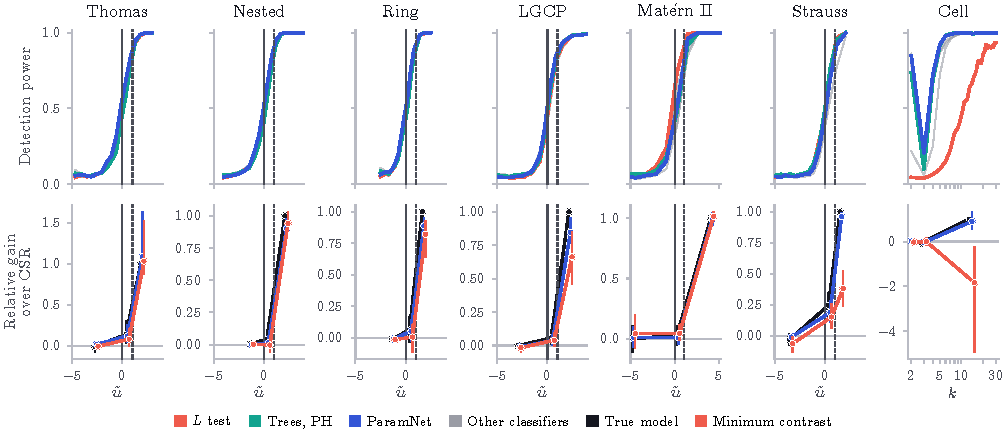
\includegraphics[width=\textwidth]{figs/v2/s_regime_detect}
\caption{Figure~\ref{fig:regime} per family; $x$ as there, cell against $k$. Top: detection power on the test
patterns of the $L$ test, trees on persistence summaries alone and ParamNet, and in grey every other classifier, all
tests of size $5\%$. Bottom: gain over CSR of the true model, ParamNet and minimum contrast on each stratum of the
evaluation set, as a share of the true model's gain in the family's strongest stratum (cell: $k\ge5$); $95\%$
bootstrap intervals over patterns. The $L$ test detects cell at its nominal $5\%$ for $k\le4$ and in $21\%$ of
patterns at $k=5$--$9$, where the learned detectors already detect almost all. Minimum contrast never selects cell,
and its fits to cell patterns at $k\ge5$ do worse than CSR.}
\label{fig:regime-detect}
\end{figure}

\begin{figure}[t]
\centering
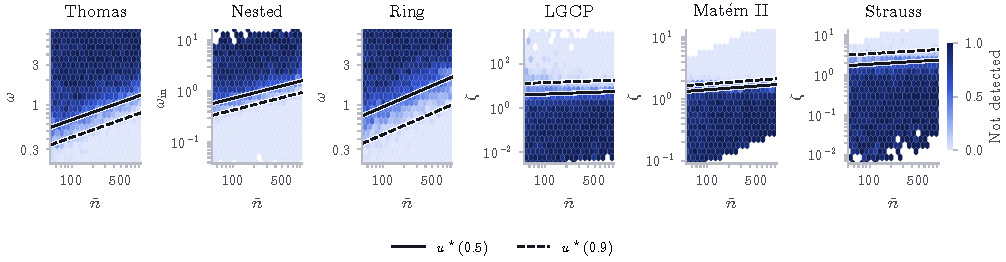
\includegraphics[width=\textwidth]{figs/v2/s_regime_map}
\caption{The boundary in the physical parameters: the share of test patterns the reference detector (trees on the
summary curves, a test of size $5\%$) does not detect, over $\nb$ and the regime coordinate $\eta$
(Table~\ref{tab:families}), with the boundary at $\tau=0.5$ (solid) and $0.9$ (dashed). Patterns approach CSR as
$\omega$ grows or $\zeta$ shrinks. Each boundary is a line $u=\log\eta+a\log\nb=u^\star(\tau)$, with slope $-a$.}
\label{fig:regime-map}
\end{figure}

\begin{table*}[t]
\caption{The regime boundary per family; regime coordinates $\eta$ as in Table~\ref{tab:families}. Detection is a
test of size $5\%$; $u=\log\eta+a\log\nb$. AUC: detection predicted from $u$ alone and from all parameters (boosted
trees, out of fold). $u^\star(0.5)$: the boundary, where detection power reaches $0.5$, fitted on the reference
detector's out-of-fold training predictions, and recomputed on the test split for the $L$ test, for trees on
persistence summaries alone (``PH only'', which never sees $L$) and for ParamNet ($95\%$ bootstrap intervals over
$\theta$). Last column: share of each family's patterns in the structured regime. Higher AUC is better. The four
boundary estimates agree to within $0.25$ in $u$ in every family. Cell has no monotone coordinate. The $L$ test
detects it at its nominal $5\%$ for $k\le4$, while trees on the summary curves already detect $84\%$ of patterns at
$k=2$ (ParamNet $85\%$): the nearest-neighbour summaries see what $K$ cannot.}
\label{tab:regime}
\begin{center}
\footnotesize
\setlength{\tabcolsep}{4pt}
\begin{tabular}{@{}lrcrcccc@{}}
\toprule
& & AUC & \multicolumn{4}{c}{Boundary $u^\star(0.5)$} & In regime \\
\cmidrule(lr){4-7}
Family & $a$ & $u$ / all & Fitted & $L$ test & PH only & ParamNet & $\tau=0.5$ / $0.9$ \\
\midrule
Thomas      & $-0.30$ & $0.935$ / $0.940$ & $-1.77$ & $-1.71$ {\scriptsize[$-1.73$, $-1.68$]} & $-1.81$ {\scriptsize[$-1.88$, $-1.77$]} & $-1.71$ {\scriptsize[$-1.74$, $-1.61$]} & $0.39$ / $0.26$ \\
Nested      & $-0.35$ & $0.950$ / $0.959$ & $-1.95$ & $-1.95$ {\scriptsize[$-2.02$, $-1.92$]} & $-2.04$ {\scriptsize[$-2.09$, $-1.98$]} & $-1.95$ {\scriptsize[$-2.01$, $-1.86$]} & $0.58$ / $0.43$ \\
Ring        & $-0.36$ & $0.928$ / $0.945$ & $-1.70$ & $-1.82$ {\scriptsize[$-1.86$, $-1.77$]} & $-1.84$ {\scriptsize[$-1.89$, $-1.77$]} & $-1.65$ {\scriptsize[$-1.79$, $-1.65$]} & $0.50$ / $0.30$ \\
LGCP        & $-0.12$ & $0.927$ / $0.936$ & $+0.91$ & $+0.95$ {\scriptsize[$+0.92$, $+1.17$]} & $+0.91$ {\scriptsize[$+0.87$, $+1.00$]} & $+0.70$ {\scriptsize[$+0.69$, $+0.92$]} & $0.31$ / $0.21$ \\
Mat\'ern II & $-0.09$ & $0.957$ / $0.962$ & $-0.05$ & $-0.09$ {\scriptsize[$-0.10$, $-0.05$]} & $+0.01$ {\scriptsize[$-0.00$, $+0.06$]} & $+0.02$ {\scriptsize[$+0.00$, $+0.03$]} & $0.42$ / $0.37$ \\
Strauss     & $-0.11$ & $0.904$ / $0.914$ & $+0.14$ & $+0.18$ {\scriptsize[$+0.13$, $+0.22$]} & $+0.14$ {\scriptsize[$+0.13$, $+0.18$]} & $+0.16$ {\scriptsize[$+0.13$, $+0.22$]} & $0.21$ / $0.11$ \\
\bottomrule
\end{tabular}
\end{center}
\end{table*}


